%%%%%%%%%%%%%%%%%%%%%%%%%%%%%%%%%%%%%%%
%  Modèle LaTeX pour les documents TB
%
%  Par Charles Duchêne, IG JI
%  Mai 2013
%
%  Toutes les images doivent se trouver
%  dans un sous-dossier pictures
%
%%%%%%%%%%%%%%%%%%%%%%%%%%%%%%%%%%%%%%%

\documentclass[12pt,a4paper]{article}
\usepackage[utf8]{inputenc} 
\usepackage[T1]{fontenc}
\usepackage[pdftex]{hyperref}	
\usepackage{amsmath}
\usepackage{amsfonts}
\usepackage[english,francais]{babel}
\usepackage{telecom}	
\usepackage{aeguill}
\usepackage{times}
\usepackage{listingsutf8}
\usepackage{makeidx}
\usepackage[style=tree,order=word,nonumberlist]{glossaries}
\usepackage{lipsum}
\usepackage{wrapfig}
\usepackage{cite}

%%%%%%%%%%
\usepackage{listings} 			% para llistas de codigo

%%%%%%%%%%%%
\makeindex
\makeglossary

%%%%%%%%%%%%%%%%%%%%%%%%%%%%
% Variables pour ce document
%%%%%%%%%%%%%%%%%%%%%%%%%%%%
\author{Lucas PEREIRA ENDRES}
\title{Developpement d'un multiplexeur MPEG2 compatible avec le standard SBTVD de télévision numérique}
%\contributors{}
\version{1.0}
\docdescription{Stage de Fin d'Études au Brésil \\ \- \\ \textbf{Tuteur:} \\ Altamiro Amadeu SUSIN \\ \textbf{Conseillers d'études:}\\ Michel JEZEQUEL et \\ Sylvie KEROUEDAN\\ 24 février à 25 juillet 2014}
%%%%%%%%%%%%%%%%%%%%%%%%%%%
%%% FICHIER DE CONFIGURATION OPTIONNEL

%%%%%%%% Propriétés pdf %%%%%%%%%%%
\hypersetup{
	bookmarks=true,
	unicode= yes,
	pdftitle={Document témoin du modèle LaTeX pour Télécom Bretagne},
	pdfauthor={Charles Duchêne},
	pdfsubject={},
	pdfkeywords={Télécom, TB, modèle, LaTeX},
	colorlinks=true,
	linkcolor=black,
	citecolor=black,
	filecolor=black,
	urlcolor = black
}

\lstset{
	basicstyle=\ttfamily\small,
	breaklines=true,
	keywordstyle=\bfseries\color{TBbrun},
	inputencoding=utf8/latin1,
}

\lstdefinestyle{stylelatex}{%
	language=tex,
	morekeywords={usepackage,newcommand,begin,renewcommand,section,
	TBannexe,TBsommaire,subsection},
	commentstyle=\itshape\color{TBvert}
}

\lstnewenvironment{latex}{%
	\lstset{style=stylelatex}}{}

\lstnewenvironment{bash}{%
\lstset{
	language=bash,
	basicstyle=\color{white}\ttfamily\small,
	keywordstyle=\color{TBvert}\bfseries,
	backgroundcolor=\color{black},
	morekeywords={sudo, cp, mkdir},
	deletekeywords={local},
}
}{}
 % fichier de configuration optionnel

\lstset{
	basicstyle=\footnotesize\ttfamily,
	%framextopmargin=50pt,
	%frame=lrtb
    language=C,
    frame=single,
    tabsize=2,
    showspaces=false,
    showstringspaces=false,
    keywordstyle=\color{blue},
    %morekeywords={QStringList,QDate,QString,QIODevice},
    commentstyle=\color{CadetBlue},
    %caption={Zistenie, či sme v daný deň, už záznam o rýchlosti uložili},
    breaklines=true
	}

%%%% DÉBUT DOCUMENT
\begin{document}
% ne pas modifier ! imprime la première page du document
\TBfrontcover
\newpage
%%%%%%%%%%%%%%%%%%%%%%%%%%%%
%     CORPS DU DOCUMENT
%%%%%%%%%%%%%%%%%%%%%%%%%%%%
 
\newpage
\section*{Résumé}
La télévision est, parmi les médias de diffusion, le plus important au Brésil. Au début de la dernière décennie, il a été décidé de numériser le système de diffusion de télévision brésilienne. Une action du gouvernement en rejoignant des entreprises et chercheurs de tout le pays a réalisé une étude sur plusieurs sujets de la télévision
numérique. Codage vidéo et audio, ainsi que les sous-systèmes d’interactivité, de multiplexage, de modulation et de transmission sont parmi les aspects étudiés du
système Numérique. Ce qui est ressorti est le SBTVD, le standard de télévision numérique brésilien, qui est basé sur la norme de transmission japonaise, ISDB-T, et
adopte H.264 et HE-AAC comme standards de codage vidéo et audio. Aujourd’hui, la quasi-totalité de l’Amérique du Sud et certains pays africains ont adopté le SBTVD.
L’objectif principal de ce travail est de développer un outil qui crée un flux de transport conforme à la norme brésilienne ABNT NBR15603, à sa fois basée sur la
norme ISO/IEC 13818-1. Pour atteindre cet objectif, une recherche considérable a été réalisée pour comprendre les concepts fondamentaux introduits par ISO/IEC13818-1
et les différences entre cette norme et l’ABNT NBR15603. Certains outils existants génèrent des flux conformes aux normes internationales, mais ne parviennent pas à respecter les spécificités du SBTVD. Une version mise à jour du framework FFmpeg est donc proposée, qui comprend maintenant les structures de données obligatoires
de le SBTVD dans le flux de transport.

\newpage
\section*{Abstract}
Television is the most important broadcast media in Brazil. At the beginning of the last decade, it was decided to digitize the Brazilian TV broadcast system. A government action joining researchers of all around the country carried out a study on several topics of Digital TV. Video and audio coding, along with interactivity and multiplexing, modulation and transmission subsystems are among the studied aspects of the DTV System. What came out is the SBTVD, the Brazilian DTV standard, which is based on the Japanese ISDB-T transmission standard, and adopts H.264 and HE-AAC as video and audio coding standards. Nowadays, almost all South American and some African countries adopted the SBTVD. The main objective of this work is to develop a tool that creates a Transport Stream compliant to the Brazilian standard ABNT NBR15603 which is based on the ISO/IEC 13818-1 standard. To achieve this objective, considerable research was carried out to understand the fundamental concepts introduced by ISO/IEC13818-1 and the differences between this standard and the ABNT NBR15603. Some existing tools generate streams compliant to the international standards but fail to obey the Brazilian specificities. An updated version of the FFmpeg framework is therefore proposed which now includes the mandatory structures of SBTVD in the Transport Stream.


%% Affichage des listes et tables.
\newpage
\listoffigures  % commenter pour ne pas avoir la liste des figures
\listoftables   % commenter pour ne pas avoir la liste des tables
\newpage
\TBsommaire

\section*{Avertissement / Disclaimer}

\-\newline
Ce travail a été élaboré basé sur la collection de logiciels FFmpeg \cite{ffmpeg} et est soumis à la licence LGPL v2.1 \cite{gplv2}. La partie modifiée du code de FFmpeg est dans la bibliothèque «avformat», qui est le droit d'auteur (C) 2003 de Fabrice Bellard. L'encodeur H.264 utilisé pour créer les échantillons de flux vidéo de ce travail est soumis à la licence GPL et est droit d'auteur (C) 2005 de Rullgard Mans (mans@mansr.com). L'auteur est prêt à aider quiconque soit intéressé à obtenir plus d'informations sur les conditions d'octroi de licences.

\-\newline
This work was developed based on the FFmpeg\cite{ffmpeg} framework and is subject to the LGPL v2.1 Licence \cite{gplv2}. The modified part of FFMpeg code is within the 'avformat' library, which is copyright (C) 2003 of Fabrice Bellard. The H.264 encoder used to create the sample video streams in this work is licenced under the GPL v2 Licence and is copyright (C) 2005 of Mans Rullgard ( mans@mansr.com). The author is willing to help whomever is interested in obtaining further information on licencing conditions.

\-\newline
\begin{minipage}{\linewidth}
\begin{lstlisting}[]
FFmpeg is free software; you can redistribute it and/or modify it under
the terms of the GNU Lesser General Public License as published by the
Free Software Foundation; either version 2.1 of the License,
or(at your option) any later version.

FFmpeg is distributed in the hope that it will be useful, but WITHOUT
ANY WARRANTY; without even the implied warranty of
MERCHANTABILITY or FITNESS FOR A PARTICULAR PURPOSE.
See the GNU Lesser General Public License for more details.

You should receive a copy of the GNU Lesser General Public License
along with FFmpeg; if not, write to the Free Software Foundation, Inc.,
51 Franklin Street, Fifth Floor, Boston, MA 02110-1301 USA.
\end{lstlisting}
\end{minipage}

\-\newline
Les codes sources pour cette modification du code de FFmpeg sont disponibles en Internet sous le système de contrôle de versions Git, à l'addresse suivante:

\-\newline
The source code for this modification is publicly available in the Internet under Git version control system, and may be accessed via the following link:
\begin{verbatim}
https://github.com/nasall2/TCC_ffmpeg
\end{verbatim}

%%%%%% INICIO DO TEXTO PROPRIAMENTE DITO

\newpage
\section{Introduction}

Historiquement, la télévision est présente dans les maisons de la plupart des citoyens brésiliens et elle est la principale source de divertissement et d'information à la population. Au cours des 10 dernières années, les nouveaux médias numériques tels que les téléphones portables et les ordinateurs sont en cours d'adoption par la population de différentes classes sociales. Un rapport récent \cite{pnad2011} dit que, en 2011, 69 \% de la population brésilienne disposait d'une ligne de téléphone mobile. Bien que significative, la participation de ce média reste largement inférieur à celle de la télévision, dont la zone de couverture atteint 100 \% du territoire via satellite \cite{StarOne}, et environ 98 \% de la population par voie terrestre \cite{globo}. La télévision est donc la principale voie de communication à la disposition du grand public au Brésil.

Face aux évolutions des systèmes de codage de médias numériques, permettant de réduire le débit de données pour transmettre de la vidéo de qualité dans les mêmes canaux utilisés pour la télévision analogique, l'ISO e l'IEC ont développé un système de transmission numérique décrit par la norme ISO/IEC13818-1. Commercialement le système est connu sous l'acronyme qui désigne le comité formé pour le rédiger, MPEG2, ou aussi connu comme la recommandation ITU-T H.222. La spécification décrit les standards de codage et transmission de vidéo, audio et des données du système. Une caractéristique clé pour les applications de télévision, c'est qu'il est possible de diffuser des programmes audiovisuels multiples simultanément par un seul diffuseur, dans le même canal physique, permettant ainsi à l'utilisateur de sélectionner les informations qu'il souhaite recevoir parmi plusieurs services envoyés.

Au Brésil, face à l'évolution de la qualité des services de télévision payée à partir de la fin des années 1990, le gouvernement a été poussé à organiser la mise en place du système de télévision numérique terrestre. À cette époque, les opérateurs des chaînes payantes par câble ou par satellite ont débuté les transmissions numériques et il fallait standardiser les transmission numérique via terrestre à fin de faire concurrence aux services payés.

Depuis 1994, les entreprises privées et le gouvernement ont financé de la recherche et des tests techniques à fin de comparer la performance de trois systèmes de télévision numérique qui ont été connus pour être efficaces dans leurs pays d'origine à l'époque: ATSC \cite{ATSC}, développé aux Etats-Unis; DVB-T \cite{DVB}, développé par un consortium d'entreprises et utilisé aux pays européens; et ISDB, développé au Japon par ARIB \cite{ARIB}. Les trois systèmes ont des similitudes et des différences en ce qui concerne l'encodage vidéo et audio: par exemple, DVB et ISDB utilisent l'infrastructure de transport de la norme MPEG2, mais diffèrent dans les schémas de modulation. Après les évaluations, il a été déterminé que le système le plus performant pour le territoire brésilien serait basée sur ISDB, avec quelques modifications, comme indiqué dans le décret présidentiel de création du système\cite{decreto8061}.

Les différences entre l'ISDB original et la norme modifiée utilisée au Brésil concernent principalement l'encodage vidéo et la plate-forme d'interactivité. Afin de promouvoir le développement de l'industrie nationale, le gouvernement a décidé d'adopter une plate-forme open source interactive, nommée Ginga, une technologie développée principalement par des chercheurs brésiliens \cite{PUCRJ}. Grâce à cet outil, le diffuseur peut, par exemple, fournir des informations utiles à la population à faible revenu qui n'a pas d'accès à \textit{Internet}. Une application possible est un projet récemment mis au point, appelé "Brasil 4D" \cite{consultas}. Les utilisateurs peuvent prendre rendez-vous avec des médecins du service public de santé, ou planifier des réunions pour résoudre les problèmes de sécurité sociale, ou bien encore consulter les offres d'emploi en temps réel, tout cela à travers la télécommande du téléviseur. Cependant, la similitude du système brésilien à la norme internationale et le fait que les interfaces interactives ne seront pas obligatoires qu'avant 2015 a conduit à un manque d'intérêt de nombreux diffuseurs dans le développement d'applications, de sorte qu'à l'heure actuelle très peu a été investi dans la création de télévision numérique interactive sur le territoire brésilien.

Le Loi Presidentiel 8061 \cite{decreto8061} du 29 juillet 2013 établit les arrêts progressifs des transmissions analogiques par régions. Jusqu'au 31 décembre 2018, tous les émetteurs analogiques seront désactivés et les canaux doivent être libérées. Les droits d'exploitation des radio-fréquences seront ensuite remis au gouvernement, qui prévoit d'utiliser la bande de 700 MHz pour le service de téléphonie mobile 4G LTE.

Un système de télévision numérique est composé essentiellement par le groupe d'équipements présentés dans la \autoref{fig:diagrama_blocos_tvd}. Au début du flux de signal, il y a des éléments de capture de vidéo et audio, tels que des caméras et des micros. Une fois capturés, la vidéo et l'audio sont compressées et codées par des codeurs correspondants. Le résultat des codeurs sont \textit{bitstreams} standardisés appelés flux élémentaires. Une fois que les flux élémentaires quittent les codeurs, ils entrent dans le multiplexeur, où tous les flux élémentaires sont mis en paquets et intégrés dans un seul flux, appelé flux de transport, ce qui est l'objectif principal de la couche système de MPEG2. Ce qui suit est un processus clé pour la robustesse du système: le flux est protégé par l'emploi de codes de correction d'erreur pour résister au bruit du canal à trajets multiples entre le diffuseur et le récepteur. Enfin, une modulation numérique est appliqué et le flux modulé est envoyé à l'antenne.

 \begin{figure}[!h]
\centering
\caption{Schéma simplifié des flux de signal de la télévision numérique.}
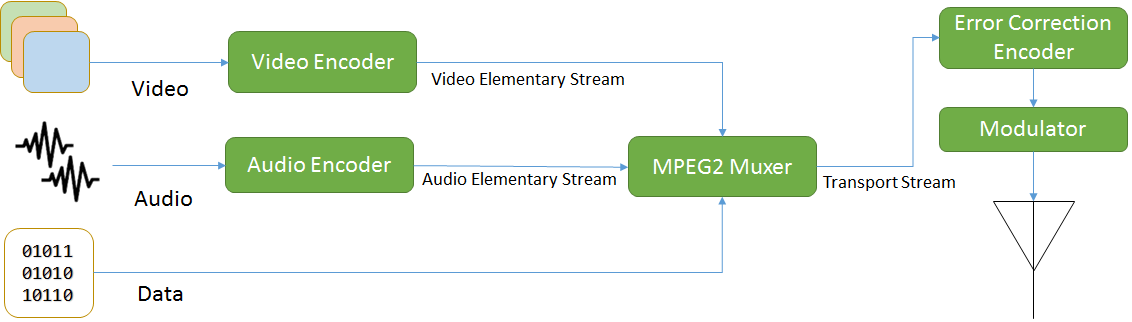
\includegraphics[width=1\linewidth]{pictures/diagrama_blocos_tvd.png}
\label{fig:diagrama_blocos_tvd}
\end{figure}
 
%La principale différence entre les systèmes de télédiffusion analogique et numérique, au niveau de la modulation, est que, dans la télévision analogique le multiplexage est dans le domaine fréquence, le signal vidéo est envoyé dans une bande de fréquence comprise dans la bande passante de canal et le signal audio dans une autre bande de fréquence. Dans la technologie numérique, le multiplexage se passe dans le domaine temporel: la sortie du multiplexeur a un débit constant, et pour les fractions de seconde seulement un paquet d'une des sources de média est envoyé à l'émetteur.

De l'autre côté du canal, le récepteur est conçu de manière à ce que, après passage de la couche de correction d'erreur, un \textit{démultiplexeur} prend le flux composé et le sépare de nouveau dans les flux binaires élémentaires. Ils sont ensuite envoyés aux décodeurs et aux dispositifs de sortie audiovisuels.

Il serait certainement troublant pour le spectateur de regarder les contenus vidéo ou audio en différé, sans synchronisation. Ainsi, un défi de ce schéma de multiplexage est de synchroniser la reproduction de tous les flux de média. Pour ce faire, des labels d'horodatage de présentation sont ajoutés périodiquement dans les flux afin qu'ils puissent être reproduits au même temps.

\section{Objectif et méthodologie}

L'objectif de ce projet est de développer un outil simple, mais flexible, pour gérer la couche des systèmes de la norme SBTVD. Fondamentalement, en utilisant cet outil on est capable de produire un fichier binaire compatible avec le système SBTVD, contenant un flux de transport qui peut être utilisé pour diffuser du contenu audiovisuel  dans des récepteurs appropriés. Beaucoup de solutions commerciales pour cet objectif sont disponibles sur le marché, de sorte que la cible ici n'était pas de développer un produit de consommation, mais plutôt quelque chose de plus académique, éducatif, où la plupart des configurations peuvent être modifiées selon les besoins. Le client interne principal à l'université (UFRGS) est l'équipe du projet appelé \textit{set-top-box} SBTVD, qui développe un boîtier décodeur du système numérique dans une architecture \textit{System on Chip} sur FPGA. Pour exécuter les tests de l'ensemble du système, les flux de transport avec différentes configurations de multiplexage doivent être diffusées à fin de tester le décodeur sur tous les cas prévus dans la norme.

Le flux de travail du projet a été séparé en trois étapes, selon le descriptif suivant. La première étape a consisté d'une recherche bibliographique à fin d'étudier la norme ABNT NBR15603, ainsi que les références y comprises à la norme ISO/IEC 13818-1 et à la norme ARIB STD-B10. Dans cette étape, l'objectif était de comprendre comment la couche Système devrait fonctionner et identifier les composants du multiplexeur qui étaient obligatoires et facultatifs. Une fois que les composants obligatoires étaient connus, les contraintes ont pu être définies. Cependant, si des structures obligatoires sont qu'à titre d'information et son absence ne bloque pas le fonctionnement du système, elles pourraient être laissés au développement futur.

La deuxième étape a envisagé définir le point de départ du développement de l'outil. Aux premières semaines de cette étape, du temps à été consacré à une recherche sur des outils existants aux repositoires d'applications \textit{open-sources} en ligne. Cela a été fait parallèlement à une évaluation de la possibilité de développer l'outil à partir de zéro, parce que d'autres chercheurs dans le laboratoire avaient déjà fait des recherches et avaient conclu que les outils libres trouvées, même avec des modifications, ne pourraient pas gérer les flux selon le standard SBTVD. Au cours de recherches menées par l'auteur lui même, des outils modifiables et avec des fonctionnalités réutilisables ont été identifiés. Ainsi, au lieu de développer à partir de zéro l'outil, il a été décidé de profiter d'un \textit{framework} existant.

Finalement, étant décidé qu'un outil existant serait modifié, la troisième étape a consisté du développement des fonctionnalités manquantes de l'outil choisie de l'étape deux, tout en respectant les contraintes définies à l'étape un, afin de la  rendre compatible avec le SBTVD. Pour valider le projet, les fonctionnalités ont été testés sur différents récepteurs.

L'objectif technique du projet est de fournir un outil qui crée des flux de transport avec trois caractéristiques principales: présentation audiovisuelle synchrone, conformité à la norme SBTVD et possibilité d'envoi de multiples services. 

TODO Ajouter la structure du laboratoire, quelques commentaires à propos du nombre d'heures,

\section{ISO/IEC 13818-1 Standard}
\label{iso13818}

The main objective of the ISO/IEC13818-1 standard is to describe the conversion of multiple bitstreams into one single stream carrying wrapped video and audio data, as well as additional information responsible to unwrap the streams. Similarly to other ISO/IEC standards, the text only specifies the decoding/demultiplexing side of the transmission chain, leaving the architectures of encoding/multiplexing stages to the manufacturers decision.

Some concepts should be briefly described to the reader by now. The first is the \textit{program} (or \textit{service}), which is formed by a collection of program elements, that on their turn are called \textit{elementary streams}. They may share a time base and then will be reproduced simultaneously. This is equivalent to the analog TV channel concept, in which a broadcaster sends a video stream and several audio streams to the viewer. The second is the \textit{PID}, which is a label assigned at the system layer to each different payload carried by the TS. Each information table has its own PID, each Elementary Stream also. The concept here is similar to a pointer, in programming: during reception of a TS packet, the demultiplexer will read the packet PID and push its payload to the appropriate buffer so that information gets concatenated with previously received packets of the same PID.

The standard defines two architectures that should be applied in different situations. The first is to be used in error free situations, such as storage in digital discs, and will not be discussed further. The other architecture, suitable for faulty, error prone transmission channels, is called the Transport Stream. The packet of this stream has fixed length and is of considerable small byte length (188 bytes), which makes it easy to error correction codes to ensure the transmission through the faulty channels. Only selected topics, that must be understood to develop the simple, but functional, MPEG-2 multiplexer of the project will be discussed in this chapter. Further information can be obtained in the full project report, in english, provided as well.

\subsection{Transport Stream Header}
\label{ts_header}

The main structure of the MPEG2 Transport Stream is a packet of constant size. The stream is made of many packets concatenated. \autoref{fig:TS_iso13818} shows the basic elements that are present in one packet, the value under each field is its length in bits. From the picture, it can be seen that a packet is roughly formed with 188 bytes of data. The mandatory header has 4 bytes, starts at the \textit{sync byte} and goes up to the \textit{continuity counter}. The packet payload may also contain the \textit{Adaptation Field}, a sort of header extension, with additional data that helps to decode and present the streams in sync. Apart from the 4 mandatory bytes of the header, the other 184 bytes may be filled with combinations of the following content: the Adaptation Field, PES data or information tables. The Adaptation Field presence is optional, and it is commonly used to carry sync data and to fill empty space in the last TS packets from one PES packet with stuffing bits.

The header fields relevant to this project are briefly described next:
\begin{itemize}
\item{The \textit{sync\hspace{0.1mm}\_\hspace{0.1mm}byte} is a fixed, 8-bit field whose value is always \texttt{0x47} and is used to identify the beginning of a TS packet;}
\item{ The \textit{payload\hspace{0.1mm}\_\hspace{0.1mm}unit\hspace{0.1mm}\_\hspace{0.1mm}start\hspace{0.1mm}\_\hspace{0.1mm}indicator} is a 1-bit field and a value of '1' indicates that either a PES packet or a PSI section starts in the current TS packet;}
\item{The field \textit{PID} is a 13-bit field, that indicates which type of data is stored in the packet payload. As will be discussed later, some PID values are reserved for specific data types;}
\item{The \textit{adaptation\hspace{0.1mm}\_\hspace{0.1mm}field\hspace{0.1mm}\_\hspace{0.1mm}control} flag is a 2-bit field and indicates if the current packet mandatory header is followed by an Adaptation Field and/or payload data. \autoref{tab_adapataion_field} gives detailed information about the values;}
\item{The \textit{data\hspace{0.1mm}\_\hspace{0.1mm}bytes} are the packet payload, and shall be contiguous bytes of data from the PES packets, PSI sections, packet stuffing bytes after PSI sections, or private data as indicated by the PID.}
 \end{itemize}

The \textit{continuity\hspace{0.1mm}\_\hspace{0.1mm}counter} is a 4-bit counter that increments on every TS packet of each individual PIDs. It works as a sequential checking and reordering information for the demultiplexer to know whether the packet order was respected in transmission, or to know if a packet was repeated. Under two conditions the continuity counter is not incremented: if a duplicate packet with payload is sent, and the \textit{adaptation\hspace{0.1mm}\_\hspace{0.1mm}field\hspace{0.1mm}\_\hspace{0.1mm}control} must be either '01' or '11' to indicate the payload presence; if there is no payload in the packet, and the \textit{adaptation\hspace{0.1mm}\_\hspace{0.1mm}field\hspace{0.1mm}\_\hspace{0.1mm}control} must be either '00' or '10'.
 
The priority indicator flag and the scrambling control flag are not used in practical implementations and were left out intentionally. However, they are part of the standard and are defined in \citeonline[2.4.3.3]{ISO}.
 
\begin{figure}[!h]
\centering
\caption{Formation scheme of a TS packet.}
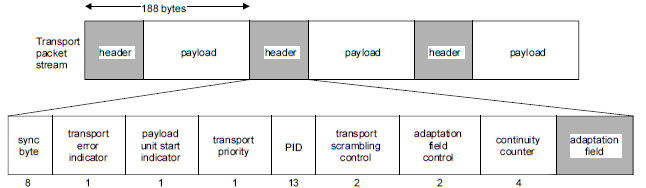
\includegraphics[width=1\linewidth]{pictures/TS_iso13818.png}
\\Source: \citeonline[F.0.1]{ISO}.
\label{fig:TS_iso13818}
\end{figure}

\begin{table}[!h]
\caption{Adaptation Field control values.}
\begin{center}
\begin{tabular}{|c|c|}
\hline
Value & Description \\
\hline
00 & Reserved for future use\\
\hline
01 & No adaptation\hspace{0.1mm}\_\hspace{0.1mm}field, payload only\\
\hline
10 & Adaptation\hspace{0.1mm}\_\hspace{0.1mm}field only, no payload\\
\hline
11 & Adaptation\hspace{0.1mm}\_\hspace{0.1mm}field followed by payload\\
\hline
\end{tabular}
\label{tab_adapataion_field}
\\Source: \citeonline[2.4.3.3]{ISO}
\end{center}
\end{table}

\subsection{Adaptation Field}

The Adaptation Field (AF) is an optional extension of the TS packet header. Although optional, it contains many useful information and is widely used in practical implementations to carry timing information and to fill with stuffing bytes remaining space in TS packets. \autoref{fig:AdapField_iso13818} shows the concatenation of fields in the Adaptation Field graphically. One characteristic of this extension is that many fields are optional, hence there are several flags that toggle the existence of the fields.

The \textit{adaptation\hspace{0.1mm}\_\hspace{0.1mm}field\hspace{0.1mm}\_\hspace{0.1mm}length} field has 8 bits and specifies the number of bytes in the adaptation field immediately after itself. When there is payload data sharing the TS packet with the adaptation field, this value shall be in the range 0 to 182. If there is no payload, just the AF, the length must be set to 183. For TS packets carrying PES data, stuffing is usually needed in the last TS packet used because PES packets are not necessarily multiples of 188 bytes. Stuffing is accomplished by setting the adaptation field length to more than the sum of the lengths of the data elements in it, so that the remaining payload bytes in PES data exactly fits in the left space. The extra space in the adaptation field is filled with stuffing bytes with the value \texttt{0xFF}.

The \textit{PCR\hspace{0.1mm}\_\hspace{0.1mm}flag} informs the presence of the optional PCR timing information in the \textit{program\hspace{0.1mm}\_\hspace{0.1mm}clock\hspace{0.1mm}\_\hspace{0.1mm}reference\hspace{0.1mm}\_\hspace{0.1mm}base} and \textit{program\hspace{0.1mm}\_\hspace{0.1mm}clock\hspace{0.1mm}\_\hspace{0.1mm}reference\hspace{0.1mm}\_\hspace{0.1mm}extension} fields, that are described in \autoref{Timing}. These fields are wrapped together in \autoref{fig:AdapField_iso13818} as 'PCR', with 42 bits.The other fields will not be described because they are not crucial for the functioning of the multiplexer. However, they are part of the standard and are defined in \citeonline[2.4.3.5]{ISO}.

\begin{figure}
\centering
\caption{Graphical representation of the Adaptation Field.}
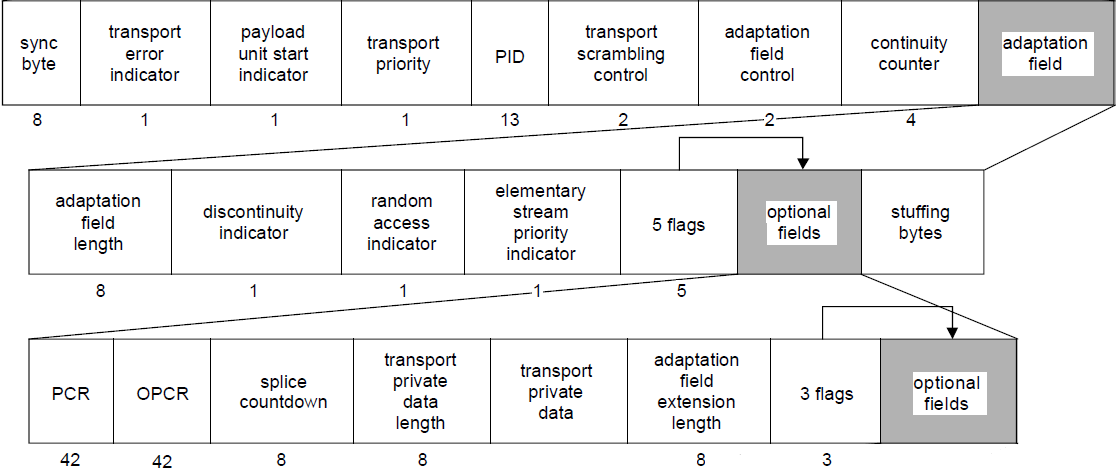
\includegraphics[width=1\linewidth]{pictures/AdapField_iso13818.png}
\\Source and Copyright: \citeonline[F.0.1]{ISO}.
\label{fig:AdapField_iso13818}
\end{figure}

\section{ABNT NBR15603 Standard}

\section{Available Solutions and Limitations}

\section{Project implementation}

\section{Tests and Results}

\section[Conclusions and Future Development]{Conclusions and Future Development}



%\subsection{}
%\subsubsection{}


% ANNEXES
\appendix
%\index{Annexe}
\TBannexe{Blah blah}
\section{Test}
\newpage
\TBannexe{Buh Buh}
\section{123}
\subsection{222}
\subsection{444}

\newpage
% INDEX, RÉFÉRENCES et GLOSSAIRE
 %\TBindex
 \TBbiblio{plain-fr}{includes/biblio}
 \TBglossary

% ne pas modifier ! imprime la dernière page du document
\TBcoverpage
\end{document}
